%Dokumentklasse
\documentclass[a4paper,12pt]{scrreprt}
\usepackage[left= 2.5cm,right = 2cm, bottom = 4 cm]{geometry}
%\usepackage[onehalfspacing]{setspace}
% ============= Packages =============

% Dokumentinformationen
\usepackage[
	pdftitle={Semesterbericht},
	pdfsubject={Wissenschaftliches Arbeiten},
	pdfauthor={Markus Weiß},
	pdfkeywords={},	
	%Links nicht einrahmen
	hidelinks
]{hyperref}



% Standard Packages
\usepackage[utf8]{inputenc}
\usepackage{float} 
\usepackage[ngerman]{babel}
\usepackage[T1]{fontenc}
\usepackage{graphicx, subfig}
\usepackage{fancyhdr}
\usepackage{lmodern}
\usepackage{color}
\usepackage{amsmath}

%Graficpath
\graphicspath{{img/}}

% zusätzliche Schriftzeichen der American Mathematical Society
\usepackage{amsfonts}
\usepackage{amsmath}

%nicht einrücken nach Absatz
%\setlength{\parindent}{0pt}


% ============= Kopf- und Fußzeile =============
\pagestyle{fancy}
%
\lhead{}
\chead{}
\rhead{\slshape \leftmark}
%%
\lfoot{}
\cfoot{\thepage}
\rfoot{}
%%
\renewcommand{\headrulewidth}{0.4pt}
\renewcommand{\footrulewidth}{0pt}

% ============= Package Einstellungen & Sonstiges ============= 
%Besondere Trennungen
\hyphenation{De-zi-mal-tren-nung}


% ============= Dokumentbeginn =============

\begin{document}

%Einrücken verhindern 
\setlength{\parindent}{0em}

%Seiten ohne Kopf- und Fußzeile sowie Seitenzahl
\pagestyle{empty}

% Beendet eine Seite und erzwingt auf den nachfolgenden Seiten die Ausgabe aller Gleitobjekte (z.B. Abbildungen), die bislang definiert, aber noch nicht ausgegeben wurden. Dieser Befehl fügt, falls nötig, eine leere Seite ein, sodaß die nächste Seite nach den Gleitobjekten eine ungerade Seitennummer hat. 
\cleardoubleoddpage

% pagestyle für gesamtes Dokument aktivieren
\pagestyle{fancy}


%===========================TITEL-Seite==============================

\title{Semesterbericht}
\date{15.01.2019}
\author{
Markus Weiß\\
Fakultät Digitale Medien,\\
Hochschule Furtwangen University\\
}
\maketitle

%Inhaltsverzeichnis
\tableofcontents

\chapter{Wissenschaftliches Arbeiten}\label{sec:parm}

\section{Forschungskonzeption}\label{sec:parm}

{\textsc{
Forschungskonzeption: Gedanklicher Entwurf eines Forschungsvorhabens\\
}}

\section{Forschungvorhaben}\label{sec:parm}

{\textsc{
Forschungsvorhaben: Wissen Generieren das wissenschaftlich begründet ist\\
}}

\section{Forschungsprojekt}\label{sec:parm}

\begin{itemize}
\item Themenfindung

\end{itemize}


\begin{itemize}
\item Strukturierung
\begin{itemize}
\item Literaturrecherche
\item Zeitplan
\item Forschungskonzeption
\end{itemize}

\end{itemize}

\begin{itemize}
\item Methoden
\begin{itemize}
\item Empirische Methoden
\item Theorien
\item Gestaltung
\end{itemize}
\end{itemize}

\begin{itemize}
\item Administratives
\begin{itemize}
\item Literatur- Quellensammlung (immer direkt übertragen)
\item Notizen- Ideensammlung
\item Sammlung von Textentwürfen (schreiben so früh wie möglich)
\end{itemize}
\end{itemize}

\begin{itemize}
\item Verfassen
\begin{itemize}
\item Texte schreiben
\item Risikopuffer
\item Rechtschreibung
\end{itemize}
\end{itemize}

\begin{itemize}
\item Controlling
\begin{itemize}
\item Neue Perspektiven
\item Forschungsfrage bzw. mit dem Ziel abgleichen
\item Abgleichen mit der Gliederung
\item Abgleichen mit dem Zeitplan
\item Risikoanalyse und Feedback einholen
\end{itemize}
\end{itemize}







\chapter{Advanced Media Production}
\section{Einführung}\label{sec:Einführung_AMP}

S3D = Stereoskopische 3D. S3D muss gerecht der visuellen Wahrnehmung produziert werden\\


\section{S3D‐Aufnahme‐, Übertragungs‐ und Darstellungstechnologien}

\subsection{Aufnahmetechnologien}
\begin{itemize}

\item Stereo‐Rendering in 3D‐Programmen und Game‐Engines: Maya Renderer, Unity S3D-Renderer
\item S3D‐Realfilm‐Kamerakonzepte 2015:
\begin{itemize}
\item 21stCentury3D/Hyperstereo
\item GoPro Dual Hero
\item P+S/Freestyle‐Spiegelrig
\end{itemize}

\end{itemize}

\subsection{Betrachtungstechnologien}
\begin{description}
\item Polfilterverfahren: Linear \& Zirkular\\
\\
	Projektoren werfen ihr Licht durch entweder recht und links zirkulierende Polfilter bis hin zur reflektierenden, Silber beschichteten Leinwand. Das Bild wird nun zurück geworfen und trifft auf die Polfilterbrille wo nun das recht drehende Licht, des rechten Bildes durch den recht gerichteten Zirkularfilter läuft und somit auf das rechte Auge trifft. Auf der linken Seite ist der Vorgang identisch.
	 
\item RGB Wellenmultiplexverfahren (z.B. CAVE-Installation) \\
\\
Hier werden die Farbinformationen nach Wellenlängen getrennt um jeweils ein rechtes und ein linkes Halbbild zu erhalten.

\item 3DTV-Polfilterverfahren
Hier werden jeweils die geraden und ungeraden Zeilen in die entgegengesetzte Richtung zirkular ausgerichtet.

\item 3DTV-Shutterverfahren
Auf dem Display wird jeweils das rechte und im Anschluss das rechte Bild angezeigt. Mit einer über Infrarot synchronisierte Shutterbrille wird jeweils das eine oder andere Auge zeit synchron das Bild erhalten.

\item Anaglyphen-Verfahren
Die linke Seite der Brille ist cyan, die rechte magenta gefärbt ...?

%=============================%
\item autostereoskope Displays\\
\begin{description}
\item Prallax‐Barriere Display\\
...
\item Lentikular Display
...
\end{description}
Script Folie 107
\item VR-Headset
\end{description}

\subsection{Displayspeisung->Bildorganisation}
\begin{itemize}
\item Frame Packing \textit{progessiv, interlace} \\

\item Side-by-Side \textsubscript{(Half)*}

\item Top-and-Bottom \textsubscript{(squeezed)*}
\end{itemize}

\subsection{Unser Auge ist keine Kamera}

\textbf{Gemeinsamkeiten von Kamera und Auge:}\\ 

\begin{table}[H]
\centering
\begin{tabular}{|r|l|}
Kamera & Auge \\
Blende & Iris \\
Sensor & Zapfen, Stäbchen \\
Fokusfunktion & Fokusfunktion \\
\end{tabular}
\end{table}


\textbf{ Was sie nicht gemeinsam haben:}\\
\begin{itemize}
\item Die Kamera hat:
\begin{itemize}
	\item eine Zoomfunktion.
	\item ist auf dem Sensor überall gleich Scharf.
\end{itemize}
\item Das Auge hat:
\begin{itemize}
	\item mehr Freiheitsgrade. Drei von den Muskeln + Kopfbewegung.
\end{itemize}
\end{itemize}



\textbf{Weitere Eigenheiten des Auges:} \\
\begin{itemize}
\item \textbf{Pupille \& Iris:}\\
Diese öffnet sich bei schwachem, und schließt sich bei starkem Lichteinfall.

\item \textbf{Zapfen:} \textit{Hellsehen, Scharfsehen} 

\begin{itemize}
	\item Zapfen sitzen ausschließlich in der Fovea Centralis
	\item Arbeiten ab ca. 1 clr/m\textsuperscript{2}	
	\item Es existieren drei Arten von Zapfen:
\begin{enumerate}
	\item SW: Short Wave
	\item MW: Medium Wave
	\item LW: Long Wave
\end{enumerate}
\end{itemize}

\item \textbf{Stäbchen:}  \textit{Dunkelsehen}
\begin{itemize}
	\item Arbeiten ab ca. <1 clr/m\textsuperscript{2}
	\item Stäbchen befinden sich überall anders, sind aber nach außen hin zu rezeptiven Feldern zusammengefasst. \textit{Siehe weiter unten Rezeptive Felder: }
	\item Zapfen 
\end{itemize}
\end{itemize}


\begin{itemize}

\item \textbf{Muskuläre Steuerung:}\\
Unserer Augäpfel sind muskulär steuerbar (3 Freiheitsgrade,
s.a. Folie 28) und im Blickfeld frei beweglich, zusätzlich
unterstützt durch Kopfbewegungen (Folie 30).

\item \textbf{Akkommodation:} \\
Die Linse in unserem Auge verändert ihre Brennweite durch muskuläre Dehnung/Streckung Ziel: maximale Schärfeabbildung eines gewünschten Fixationspunkts auf die fovea centralis -> Akkommodation.
Fokussierungen -> 4m Abstand -> Ziliarkörper ist komplett entspannt. Linse ist in den Zonularfasern natürlich aufgespannt (dünn) Fokussierungen < 2m Abstand führen zu deutlich „spürbaren“ Ziliarkontraktionen. Linse wird in den Zonularfasern entspannt (dick)

\item \textbf{Rezeptive Felder:} \textit{(Bestehend aus Stäbchen)}\\ 
 Die Rezeptoren auf der gekrümmten Netzhaut sind zusammengeschaltet zu „Rezeptiven Feldern“, welche mit zunehmenden Abstand vom Sehzentrum immer größer werden. Ein Nervenimpuls wird nur bei Helligkeitsdifferenzen innerhalb des Feldes ausgelöst des weiteren werden die rezeptiven Felder zur Kantenerkennung genutzt(Hell, Dunkel Kontraste).

\item \textbf{Fovea zentralis:}\\
Zentraler Schärfebereich (fovea centralis) und temporales / nasales Gesichtsfeld werden im Gehirn getrennt verarbeitet (s. Folie 34). Erkennung von Kanten und Bewegung Fluchtreflex
\end{itemize}


\subsection{Natürliche Okulomotorik}

Unser natürliches Sehen ist geprägt von einem Konvergenz-zu-Akkomodations-Verhältnis (C/A)-Ratio von $\approx$ 1:1

\begin{itemize}

\item \textbf{Konvergenz:} Das Eindrehen der Augen
\item \textbf{Fixation:} Konvergieren zum Kreuzungspunkt
\item \textbf{Akkommodation:} Ist die Konvergenz im Gange versuchen \textit{gleichzeitig} Ziliarmuskeln den Brechungsindex der Augenlinsen Reflexhaft anzupassen
\item \textbf{Okulomotorische Stereopsis:} Zerebrales Feedback der muskulären Spannungen von Konvergenz \&	Akkommodation und Abgleich mit erlerntem, absolutem Entfernungswissen aus Ringmuskel und Augenmuskeln. (Funktioniert aber nur bis ca. 2m Entfernung, Das Hirn kann sich Anhand der Muskelspannung den Abstand merken)

\item \textbf{Da wo wir hin konvergieren da Akkomodieren wir auch. im Verhältnis von 1:1}

\end{itemize}


\section{Warum sehen wir die Welt nicht doppelt}


\subsection{Wie nehmen wir unsere Umwelt war}
\textbf{ Unser Blickfeld besteht aus drei unter Kategorien:}

\begin{itemize}
\item  \textbf{Blickfeld 1:}
Bereich höchster örtlicher Auflösung -> optimiert auf Detailwahrnehmung
\item  \textbf{Blickfeld 2:}
Bereich differenzieller Grobverarbeitung -> optimiert auf Strukturwahrnehmung
\item  \textbf{Blickfeld 3:} 
Bereich flächiger, temporaler Verarbeitung -> optimiert auf Bewegungswahrnehmung
\end{itemize}

\textbf{Merksatz:} \\

Nur eine schmaler Bereich unserer visuellen Wahrnehmung realisiert hohe örtliche Auflösung.
Die übrigen Bereiche sind evolutionär optimiert auf die Erkennung von Grobstrukturen und Bewegungen!
Erst durch die Summe der muskulären Augensprünge („Saccaden“) mit jeweiliger Akkommodation auf die
Fixationspunkte ergibt sich die scharfe Gesamtwahrnehmung unserer Umgebung.

\subsection{Exkurs zur Selektiven Schärfe}

\begin{itemize}
\item Unscharfe Bildbereiche „vertreiben“ das Auge des Zuschauers
(keine Möglichkeit der scharfen Fixation ‐ selbst bei extremem Bemühen des Zuschauers)
\item Szenische Anwendung: „Selektive Schärfe“
Schärfe/Unschärfe wird klassisch ganz bewusst zur gezielten Lenkung und Bindung der Aufmerksamkeit der Zuschauer eingesetzt.
\end{itemize}

\textbf{Tiefenschärfe:}
Ist abhänging von: 
\begin{itemize}
\item Kamera‐/Focal‐Abstand a zur Szene
\item gewählte Brennweite \textit{f} 
\item Verhältnis Brennweite/Bildsensorgröße
\item Blendenzahl \textit{k} 
\end{itemize} 

\textbf{Funktionert das Prinzip der „selektiven Schärfe“ auch in VR-Produktionen?}
Durch die 3D-Umgebung hat der Mensch nun die Möglichkeit sich seinen Bereich von Interesse selbst zu suchen. Hier eine Unschärfe einzubauen würde eher zu einer negative empfundenen Erfahrung führen. \\

\subsection{Warum wir die Welt nicht doppelt sehen}

\subsubsection{Zyklopische Fusion}

\begin{figure}[H] 
  \centering
	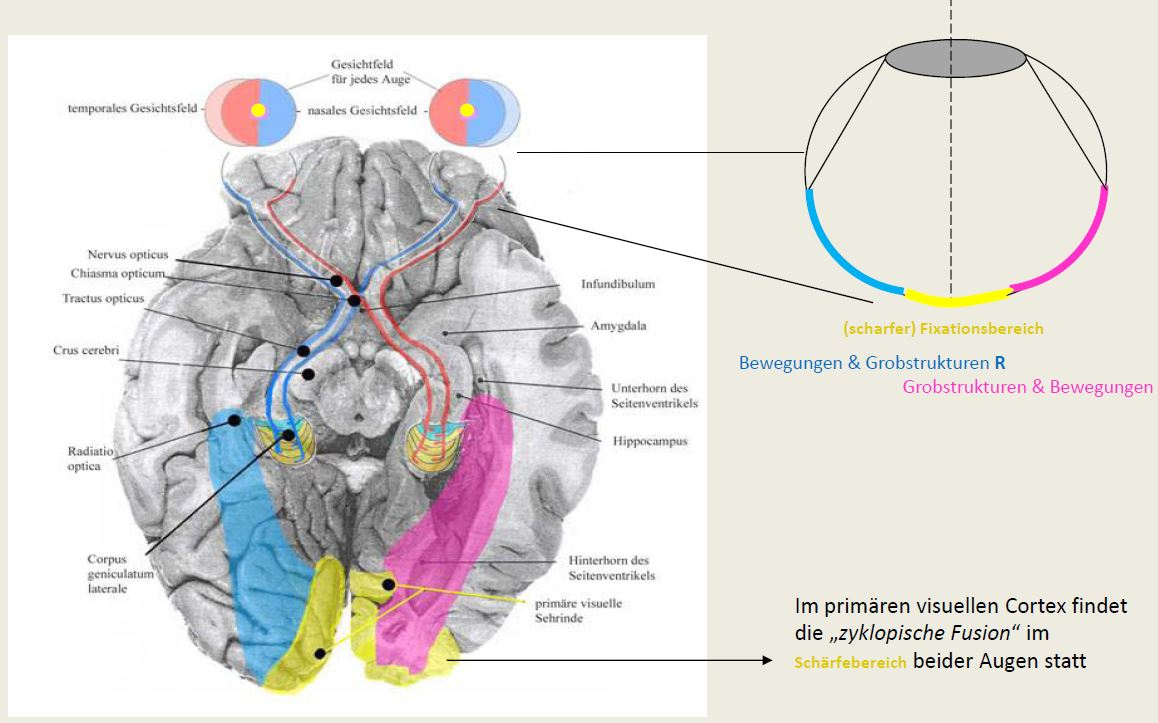
\includegraphics[width=15cm]{AdvancedMediaProduktion/ZyklopischeFusion.JPG} 
  \caption{Zyklopische Fusion}
  \label{fig:Bild1}
\end{figure}

\subsection{Patente Stereopsis}

\subsubsection{Binokulare Querdisparität}

\subsubsection{Fixationsdisparität}

\subsubsection{Stereosehen ist Zapfensehen}

\subsubsection{Medizinischer Nachweis}

\subsubsection{Patente Stereopsis: Der schmale Grat der auswertbaren Fixationsdisparität}

\subsubsection{Patente Stereopsis: Der schmale Grat der verträglichen Fixationsdisparität beim Menschen}

\subsubsection{Patente Stereopsis ist nur im sog. „Panumraum“ möglich}
\textbf{Horopter} = Linie gleich wahrgenommener Entfernung bei variabler Augenbewegung aber unverändertem Akkommodationsabstand a.\\
\textbf{Panumraum} = Summe aller stereoptisch wahrnehmbaren Raumsegmente auf dem jeweiligen Akkommodations‐Horopter.\\

\begin{figure}[H] 
  \centering
	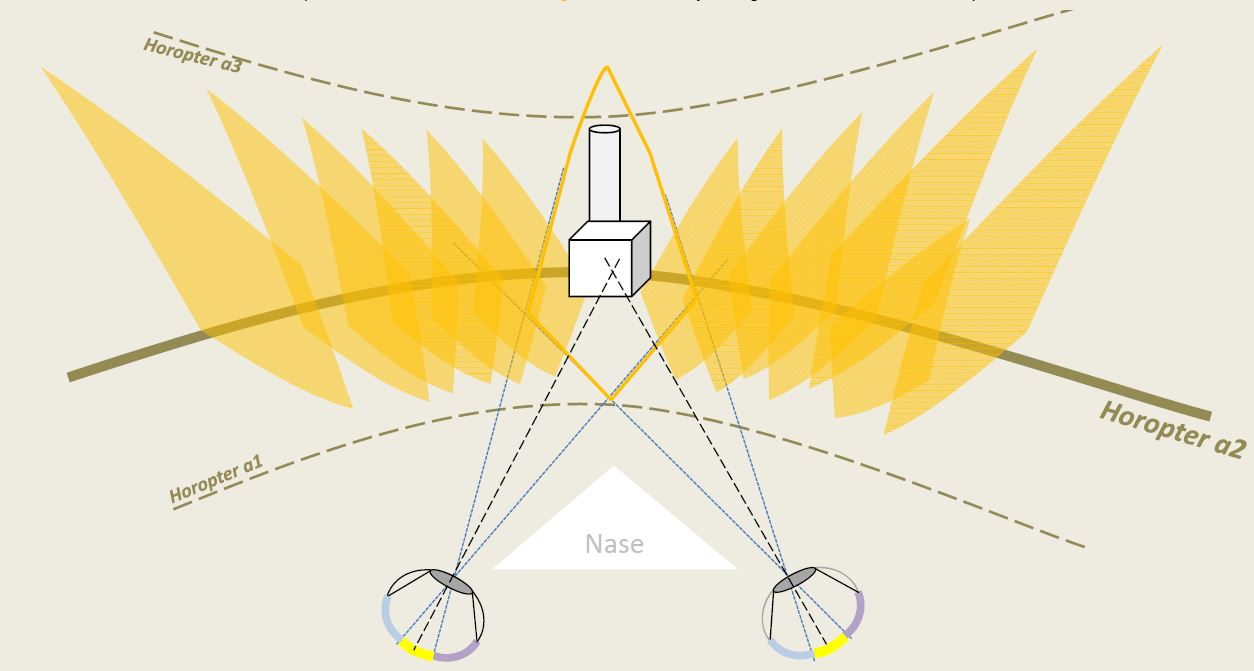
\includegraphics[width=15cm]{AdvancedMediaProduktion/Panumraum.JPG} 
  \caption{Panumraum}
  \label{fig:Bild2}
\end{figure}


\subsubsection{Grenzen der binokularen Fusionfähigkeit / Summation}

\textit{Binokulare Fusion} =

\textbf{Schwache Unterschiede}
\textbf{Erhöhte Unterschiede}
\textbf{Massive Unterschiede}



\subsubsection{Patente Stereopsis ist NICHT kanten‐ oder objekt‐ sondern mehrheitlich punktgetrieben}

\subsubsection{Warum können Menschen mit einer Augenklappe trotzdem problemlos Autofahren?}
Die menschliche Tiefeninterpretation stützt sich auf mehrere Hinweisreize („depth cues“) ab!
Die Stereopsis ist nur EIN Hinweisreiz für die menschliche Tiefeninterpretation!\\


\subsection{Monokulare depth cues}

\subsubsection{Verdeckung}
\subsubsection{Atmosphärische Perspektive}
\subsubsection{Perspektivische Konvergenzen}
\subsubsection{Gewohnte Größe im Blickfeld}
\subsubsection{Relative Größe im Blickfeld}
\subsubsection{Relative Höhe im Blickfeld}
\subsubsection{Licht \& Schatten}
\subsubsection{Texturdichte‐gradient)}
\subsubsection{Bewegungsparallaxe}
\subsubsection{Dynamische Verdeckung}







\chapter{Formale Sprachen}\label{sec:Kapitel formale Sprachen}
\section{Grundlagen der Mengenlehre}\label{sec:Einführung_FS}

\textbf{Kapitelinhalt:}
\begin{itemize}
\item Grundlagen der Mengenlehre
\item Relationen und Funktionen
\item Die Welt der Zahlen
\item Rekursion und induktive Beweise 
\end{itemize}


\subsection{Der Mengenbegriff}


\begin{figure}[h]
\centering
\textit{a} $\in$ M,\\ bedeutet a ist \textbf{ein} Element der Menge \textit{M}.\\
\textit{a} $\notin$ M,\\ bedeutet a ist \textbf{kein} Element der Menge \textit{M}.\\
\textit{a,b} $\in$ M,\\ bedeutet, dass a und b \textbf{ein} Element der Menge \textit{M} sind.\\
\textit{a,b} $\notin$ M,\\ bedeutet, dass a und b \textbf{keine} Element der Menge \textit{M} sind.\\

\textit{M}\textsubscript{1} und \textit{M}\textsubscript{2} gelten als \textbf{gleich}\\ 
(\textit{M}\textsubscript{1} $=$ \textit{M}\textsubscript{2}),\\
 wenn sie \textbf{exakt} dieselben Elemente enthalten.\\

\textit{M}\textsubscript{1} und \textit{M}\textsubscript{2} gelten als \textbf{ungleich}\\ 
(\textit{M}\textsubscript{1} $\neq$ \textit{M}\textsubscript{2}),\\
 wenn sie \textbf{exakt} dieselben Elemente enthalten.\\

Auch eine \textit{leere} Menge, gilt als Menge und wird mit $\emptyset$ symbolisiert.\\
 
In einer Menge ist \textbf{niemals zweimal} das selbe Element enthalten und besitzen auch keinen festen Platz. Sie sind somit \textit{inhärent} und \textit{ungeordnet}.\\

\end{figure}


\newpage    

\textbf{Zeichenerklärung:}\\

\textbf{Runde Klammern:}\\

\begin{figure}[h]
\centering
{(...)} = Tuple o. Paar.\\ 
\end{figure}

(\textit{Hinweis:} In Runden Klammern ist die Reihenfolge entscheidet. D.h. das dieses Paar auch nur genau so als Menge vorkommen darf )\\

\textbf{Geschweifte Klammern:} \\ 

\begin{figure}[h]
\centering
\{...\} = Aufzählung. \\ 
\end{figure}

(\textit{Hinweis:} Bei einer Aufzählung von Mengen ist die Reihenfolge egal.\\




\textbf{Aufzählende Beschreibung}\\
Die Elemente einer Menge werden explizit aufgelistet. Selbst unendliche
Mengen lassen sich aufzählend \textit{enumerativ} beschreiben,
wenn die Elemente einer unmittelbar einsichtigen Regelmäßigkeit
unterliegen. Die nachstehenden Beispiele bringen Klarheit:\\

Die Menge der \textit{natürlichen Zahlen}: \\

\begin{figure}[h]
\centering

$\mathbb{N}$ := \{0,1,2,3,... \}\\
\textit{M}\textsubscript{1} := \{0,1,2,3,... \}\\
\end{figure}

\textbf{Deskriptive Beschreibung}\\
Die Mengenzugehörigkeit eines Elements wird durch eine charakteristische
Eigenschaft beschrieben. Genau jene Elemente sind in der
Menge enthalten, auf die die Eigenschaft zutrifft.\\

\begin{figure}[h]
\centering
\textit{M}\textsubscript{3} := \{ \textit{n} $\neq$ $\mathbb{N}$ | \textit{n} mod 2 = 0 \}\\
\textit{M}\textsubscript{4} := \{ \textit{n} \textsuperscript{2} | $\neq$ $\mathbb{N}$  \}\\
\end{figure}

Demnach enthält die Menge \textit{M}\textsubscript{3} alle Elemente \textit{n} $\in$ $\mathbb{N}$, die sich ohne
Rest durch 2 dividieren lassen, und die Menge \textit{M}\textsubscript{4} die Werte \textit{n} \textsuperscript{2} für alle natürlichen Zahlen \textit{n} $\in$ $\mathbb{N}$. Die Mengen \textit{M}\textsubscript{3} und \textit{M}\textsubscript{4} sind damit nichts anderes als eine deskriptive Beschreibung der im vorherigen
Beispiel eingeführten Mengen \textit{M}\textsubscript{1} und \textit{M}\textsubscript{2}.\\

\textbf{Teilmengenbeziehungen:}
\begin{figure}[H]
\centering

$\subseteq$ = ist Teilmenge von:\\ 
\textit{M}\textsubscript{1} $\subseteq$ \textit{M}\textsubscript{2} 
$\Leftrightarrow$ 
Aus \textit{a} $\in$ \textit{M}\textsubscript{1} flogt \textit{a} $\in$ \textit{M}\textsubscript{2}\\


$\supseteq$ = ist Obermenge von:\\
\textit{M}\textsubscript{1} $\subseteq$ \textit{M}\textsubscript{2}
$\Leftrightarrow$ 
\textit{M}\textsubscript{2} $\supseteq$ \textit{M}\textsubscript{1}\\

\end{figure}


\subsection{Mengenoperationen}


\textbf{Vereinigung:}\textit{M}\textsubscript{1} vereinigt mit \textit{M}\textsubscript{2}\\
\textit{M}\textsubscript{1} $\cup$ \textit{M}\textsubscript{2} :=  \\
\{ \textit{a} | \textit{a} $\in$ \textit{M}\textsubscript{1} oder \textit{a} $\in$ \textit{M}\textsubscript{2} \}


\textbf{Schnitt:} \textit{M}\textsubscript{1} (herraus)geschnitten \textit{M}\textsubscript{2} 
\textit{M}\textsubscript{1} $\cap$ \textit{M}\textsubscript{2} :=  \\
\{ \textit{a} | \textit{a} $\in$ \textit{M}\textsubscript{1} und \textit{a} $\in$ \textit{M}\textsubscript{2} \}


\textbf{Differenz:} Die Differenz meint die Menge, den Anteil von \textit{M}\textsubscript{2} aus \textit{M}\textsubscript{1} entfernt.
\textit{M}\textsubscript{1} $\cap$ \textit{M}\textsubscript{2} :=  \\
\{ \textit{a} | \textit{a} $\in$ \textit{M}\textsubscript{1} und \textit{a} $\in$ \textit{M}\textsubscript{2} \}


\textbf{Komplement:} Die Komplementmenge, meint die Menge, die übrig bleibt wenn man alles weg lässt außer \textit{M}\textsubscript{1}.\\



\newpage
\subsubsection{Mengenalgebra}

\textbf{Kommunikativgesetze:} Meint, es ist egal wo eine Menge steht, die Operation ist die selbe.\\
\begin{figure}[H]
\centering
\textit{M}\textsubscript{1} $\cap$ \textit{M}\textsubscript{2} = 
\textit{M}\textsubscript{2} $\cap$ \textit{M}\textsubscript{1}\\

\textit{M}\textsubscript{1} $\cup$ \textit{M}\textsubscript{2} = 
\textit{M}\textsubscript{2} $\cup$ \textit{M}\textsubscript{1} \\
\end{figure}


\textbf{Distributivgesetze:} Meint, das eine Menge immer in eine Klammer hinein multipliziert werden kann. Wobei hier die Operatoren in der Klammer umgedreht werden müssen.\\
\begin{figure}[H]
\centering
\textit{M}\textsubscript{1} $\cup$ ( \textit{M}\textsubscript{2} $\cup$ \textit{M}\textsubscript{3}) =
(\textit{M}\textsubscript{1} $\cup$ \textit{M}\textsubscript{2}) $\cap$ (\textit{M}\textsubscript{1} $\cup$ \textit{M}\textsubscript{3})
\end{figure}


\textbf{Neutrales Element:} Das neutrale Element meint, eine Menge vereinigt mit der leeren Menge, ist die Menge selbst. Eine Menge geschnitten mit dem Komplement, ist auch die Menge selbst. \\
\begin{figure}[H]
\centering
\textit{M} $\cup$ $\emptyset$ = \textit{M}\\
\textit{M} $\cap$ \textit{T} = \textit{M}
\end{figure}




\textbf{Inverse Elemente:} Das inverse Element einer Menge ist, eine Menge vereinigt mit seiner \textit{Komplementärmenge} ist das \textit{Komplement}. Eine Menge geschnitten mit seiner Komplementärmenge, ist die \textit{leere Menge}.\\
\begin{figure}[H]
\centering
%\textit{M} $\cup$ \overline{\textit{M}} = \textit{T}\\
%\textit{M} $\cap$ \overline{\textit{M}} = $\emptyset$
\end{figure}

\textbf{Assoziativgesetze:} Meint, dass wenn auf alle Mengen einer Gleichung die selbe Operation durchgeführt wird, tritt wieder das Kommunikativgesetz in Kraft. Gilt also auch für Vereinigung wie auch für Schnitt\\
\begin{figure}[H]
\centering
\textit{M}\textsubscript{1} $\cup$ (\textit{M}\textsubscript{2} $\cup$ \textit{M}\textsubscript{3}) = 
(\textit{M}\textsubscript{1}) $\cup$ \textit{M}\textsubscript{2}) $\cup$ \textit{M}\textsubscript{3}\\
\end{figure}

\textbf{Idempotenzgesetze:} Eine Menge, geschnitten oder vereinigt mit sich selbst ist immer die Menge selbst.\\
\begin{figure}[H]
\centering
\textit{M} $\cup$ \textit{M} = \textit{M}\\
\textit{M} $\cap$ \textit{M} = \textit{M}\\
\end{figure}

\textbf{Absorptionsgesetze:} Eine Menge \textit{vereinigt} mit einem \textit{Schnitt} derselben Menge und einer anderen Menge ergibt die Menge selbst. Eine Menge \textit{geschnitten} mit einer \textit{Vereinigung} derselben Menge und einer anderen Menge ist auch die Menge selbst. \\
\begin{figure}[H]
\centering
\textit{M}\textsubscript{1} $\cup$ (\textit{M}\textsubscript{1} $\cap$ \textit{M}\textsubscript{2}) = \textit{M}\textsubscript{1}\\ 
\textit{M}\textsubscript{1} $\cap$ (\textit{M}\textsubscript{1} $\cup$ \textit{M}\textsubscript{2}) = \textit{M}\textsubscript{1}\\ 
\end{figure}

\textbf{Gesetze von De Morgan:} Das \textit{Komplement} einer Operation ist immer die gegenteilige Operation\\
%\begin{figure}[H]
%\centering
%\overline{\textit{M}\textsubscript{1} $\bar{\cup}$ \overline{\textit{M}\textsubscript{2}} = 
%\overline{\textit{M}\textsubscript{1}} $\cap$ \overline{\textit{M}\textsubscript{2}}
%\end{figure}

\textbf{Auslöschungsgesetze:} \\
Eine Menge vereinigt mit der \textit{Komplementärmenge} ist die Komplementärmenge.\\
\begin{figure}[H]
\centering
\textit{M} $\cup$ \textit{T} = \textit{T}\\
\end{figure}
Eine Menge geschnitten mit der neutralen Menge ist die neutrale Menge.\\
\begin{figure}[H]
\centering
\textit{M} $\cup$ $\emptyset$ = $\emptyset$\\
\end{figure}

\textbf{Gesetz der Doppelnegation:}\\
\begin{figure}[H]
\centering
$\overline{\overline{M}}$ = \textit{M}
\end{figure}


\textbf{Kardinalität:} Meint den Betrag deiner Menge. Also die Anzahl der Elemente einer Menge.\\
\begin{figure}[H]
\centering
\textit{M} = \{1,2,3,4\}  $\Rightarrow$ |\textit{A}| =4\\
\end{figure}

\textbf{Potenzmenge:} Meint die \textit{Vereinigung} aller Teilmengen zu einer neuen Menge 2\textsuperscript{\textit{M}}. Jede nicht leere Menge hat mindestens Zwei Elemente\\

\textit{M} = \{ \{a\}  ,\{b\} \}
\textit{P} = \{ $\emptyset$, \{a\}  ,\{b\}, \{a,b\} \}\\
2\textsuperscript{ \textit{M}} := \{ \textit{M'} | \textit{M'} $\subset$ \textit{M} \}


\textbf{Partition \& Äquivalenzklassen:} Eine \textit{Partition} von \textit{M}, ist wenn jedes Element aus M in nur einer Menge aus \textit{P} liegt. Die Elemente aus \textit{P} werden als \textit{Äquivalenzklassen} bezeichnet.\\
\textit{P} $\subseteq$ 2\textsuperscript{\textit{M}}

\section{Relationen und Funktionen}

\textbf{Zeichenerklärung:}\\
\begin{figure}[h]
\centering
\textbf{Relationalzeichen:} \textit{$\sim$} = steht in Relation zu.\\
\end{figure}

Kartesischses Produkt

\subsection{Relation}

Graphdarstellung
Matrix-Darstellung hier noch bespiel der Potentmenge als Matrix (alle möglichen kombinationen müssen abgedeckt sein)\\


Relationsattribute:
reflexiv
irreflexiv
symetisch
asymmetisch
antisymmetisch
transitiv
linkstotal
rechttotal
linkseindeutig
rechtseindeutig

Relationsprodukt, inverse Relation

Transitive Hülle

Reflexiv Transitive Hülle

Äquivalenzrelation
Ordnungsrelation


Surjetivität
Injetivität
Bijetivität


\subsection{Funktion}

Bei Funktionen kann zunächst zwischen Funktionen der Informatik und der Mathematik gesprochen werden. 

total 
partiell

surjetiv
bijetiv
bijetiv


\section{Die Welt der Zahlen}
\subsection{Natürliche, rationale und reelle Zahlen}
\subsection{Von großen Zahlen}
\subsection{Die Unendlichkeit begreifen}

\section{Rekursion und induktive Beweise}
\subsection{Vollständige Induktion}














%Verzeichnis aller Bilder
%\listoffigures

%Verzeichnis aller Tabellen
%\listoftables

\end{document}
